\documentclass[../main.tex]{subfiles}
\graphicspath{{\subfix{../images/}}}

\begin{document}

There are many ways to actually author code. There are 3 main ways of doing so.

\paragraph{Text Editors}

They are typically the most simple. They are meant to just edit \emph{plain text}, which means raw ASCII/Unicode data without any formatting data. On macOS, the default text editor is TextEdit, on Windows it is Notepad, and on Linux...it depends.

\begin{figure}[H]
    \centering
    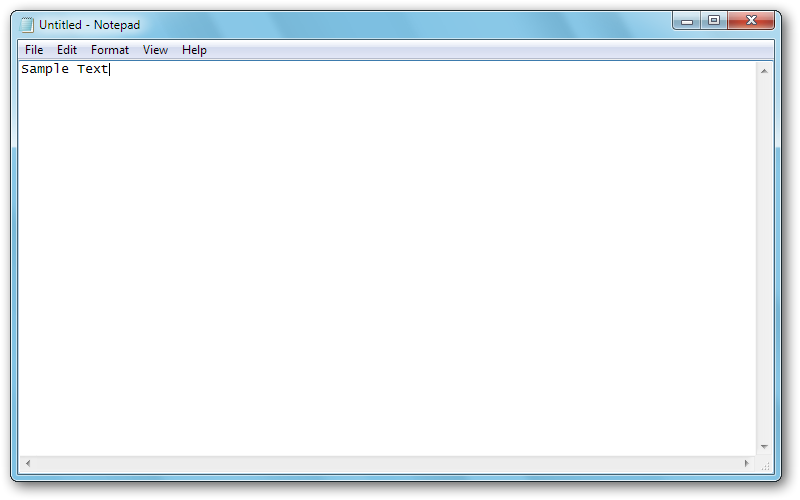
\includegraphics[width=0.7\textwidth]{windows_notepad.png}
    \caption{A screenshot of Windows Notepad.}
    \label{fig:windows_notepad}
\end{figure}

They typically do not have any convenience features for programmers, which is why people don't typically use them.

\paragraph{IDEs (Integrated Development Environments)}

These are much more sophisticated than just text editors. They are like text editors, but tailored to writing code. They usually have tabs and nice features like a compiler/interpreter built into them, a debugger, error diagnostics, autocompletion, auto-documenters/documentation generators and pretty-printing.

For a more thorough discussion on IDEs, look at page 170 on the textbook.

\paragraph{Code Editors}

These are more sophisticated than just text editors, as they have features like syntax highlighting\footnote{"fancy colors".} and coding-specific features. They are not talked about often, as most people just use IDEs. This is also not in the syllabus, but is interesting to know.

Personally, I\footnote{Eason Qin.} use {\ccmono neovim} on Linux, it is based in the terminal. It looks as follows:

\begin{figure}[H]
    \centering
    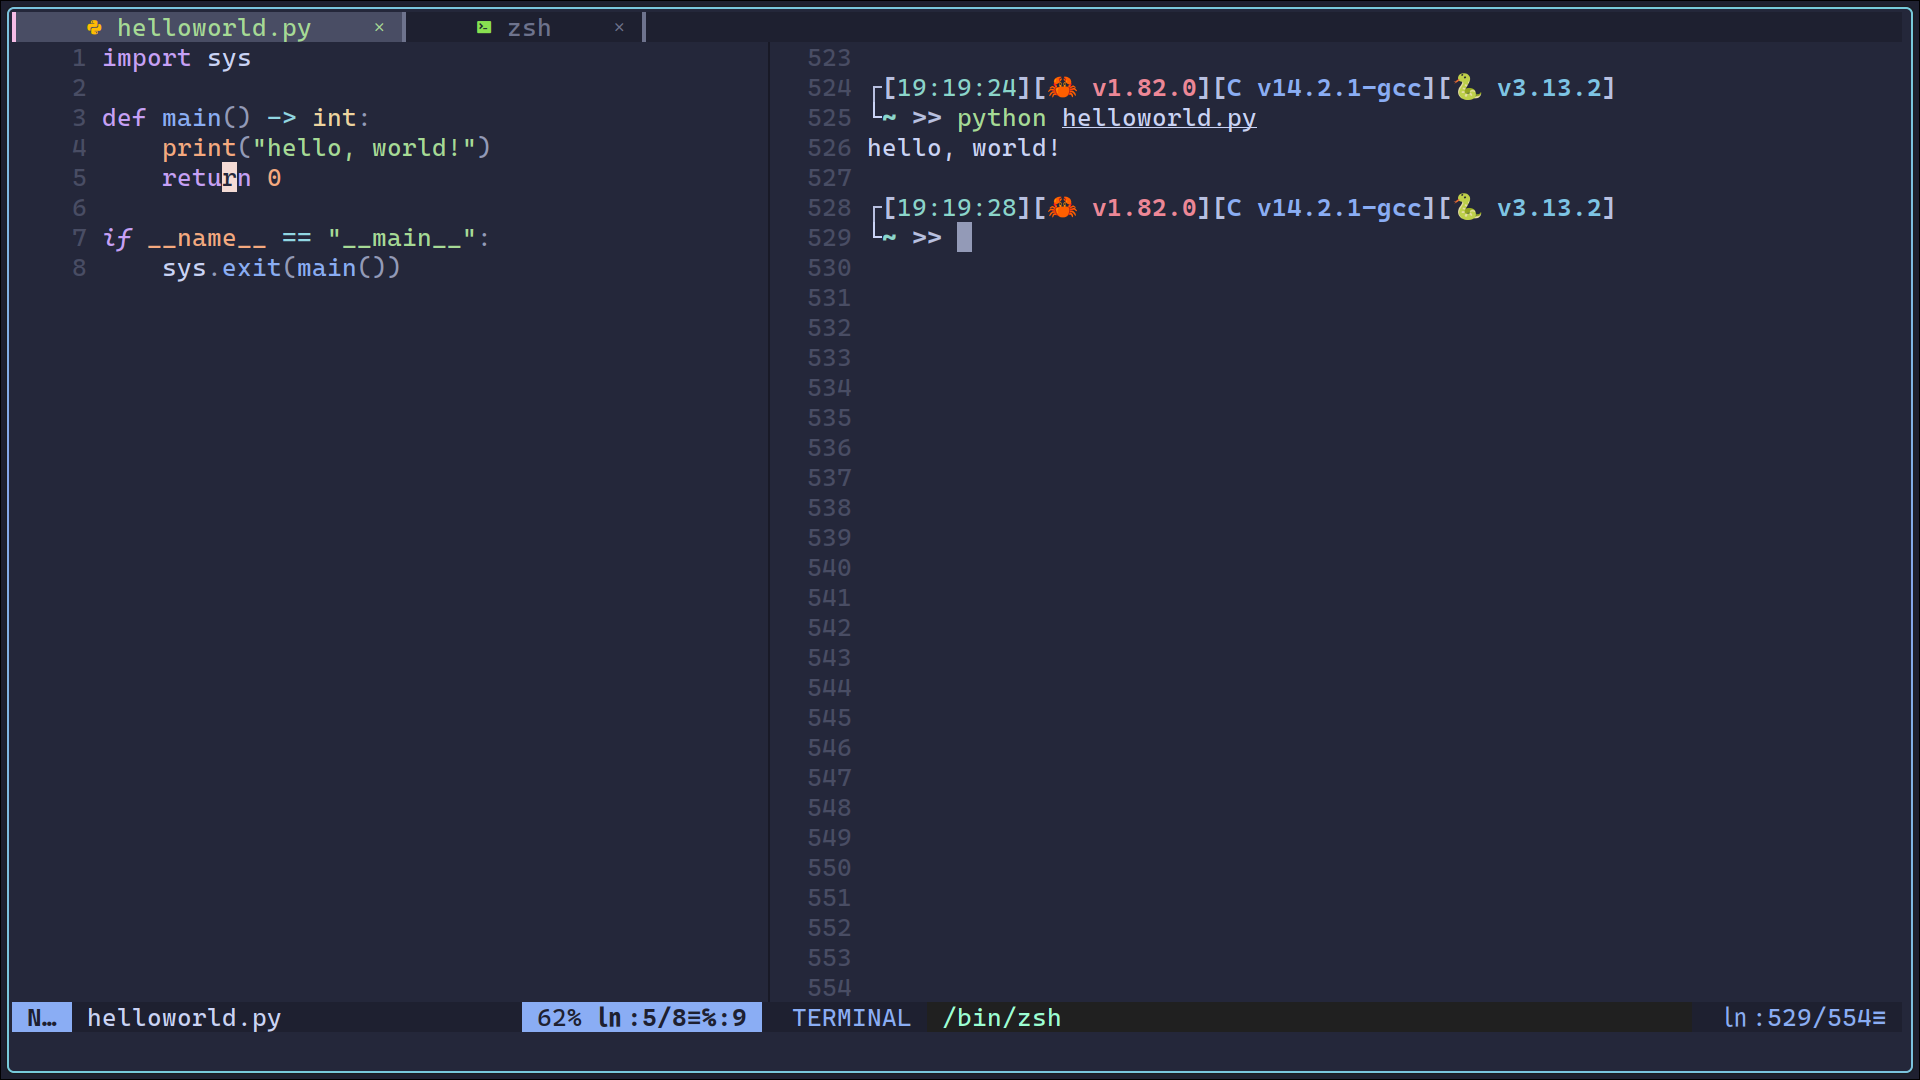
\includegraphics[width=0.7\textwidth]{code_editor.png}
    \caption{A screenshot of neovim running on Hyprland.}
    \label{fig:code_editor}
\end{figure}


\end{document}
